\documentclass[12pt,a4paper]{article}
\usepackage[utf8]{inputenc}
\usepackage[portuguese]{babel}
\usepackage[margin=2.5cm]{geometry}
\usepackage{hyperref}
\usepackage{graphicx}
\usepackage{booktabs}
\usepackage{float}

\title{Relatório Final - Laboratório 01\\ \large Características de repositórios populares}
\author{André Xavier Lazarini e João Pedro Guimarães}
\date{\today}

\begin{document}

\maketitle

\section{Introdução}

\subsection*{Contextualização e Problema Foco do Experimento}
O ecossistema de desenvolvimento de software atual depende fortemente de sistemas open-source. Entender como esses sistemas operam é fundamental para compreender as dinâmicas da comunidade de desenvolvedores. O problema central que este experimento busca analisar é como esses sistemas populares são desenvolvidos, a frequência com que recebem contribuição externa e a constância com que lançam atualizações.

\subsection*{Objetivo (Principal e Específicos)}
O objetivo principal deste laboratório é estudar as principais características de sistemas populares open-source. Para atingir esse propósito, o estudo baseia-se na coleta e discussão de dados dos 1.000 repositórios com o maior número de estrelas no GitHub. Como objetivos específicos, buscamos sumarizar esses dados através de valores medianos e contagens para extrair o perfil de um repositório de sucesso.

\subsection*{Questões-Pesquisa e Hipóteses}
Para guiar a investigação proposta neste laboratório, definimos hipóteses para cada uma das Questões de Pesquisa (RQs). Essas hipóteses são baseadas no que imaginamos encontrar antes de analisar os dados reais coletados no GitHub.

\begin{itemize}
    \item \textbf{RQ 01. Sistemas populares são maduros/antigos?}
    \textit{Hipótese:} Sim. Esperamos que a grande maioria dos repositórios no top 1.000 tenha uma idade avançada.
    
    \item \textbf{RQ 02. Sistemas populares recebem muita contribuição externa?}
    \textit{Hipótese:} Sim. Acreditamos que o número de Pull Requests aceitas será altíssimo. Projetos gigantescos dependem ativamente da comunidade.
    
    \item \textbf{RQ 03. Sistemas populares lançam releases com frequência?}
    \textit{Hipótese:} Esperamos uma alta frequência de releases. Projetos bem mantidos geralmente adotam práticas ágeis e entrega contínua.
    
    \item \textbf{RQ 04. Sistemas populares são atualizados com frequência?}
    \textit{Hipótese:} Altamente frequente. O tempo até a última atualização deve ser de poucos dias ou até horas, refletindo repositórios ativos.
    
    \item \textbf{RQ 05. Sistemas populares são escritos nas linguagens mais populares?}
    \textit{Hipótese:} Sim. Nossa expectativa é que a grande maioria dos projetos utilize as linguagens de programação mais conhecidas e requisitadas pelo mercado atual.
    
    \item \textbf{RQ 06. Sistemas populares possuem um alto percentual de issues fechadas?}
    \textit{Hipótese:} Sim. Esperamos que a maior parte das issues já estejam resolvidas e fechadas.
    
    \item \textbf{RQ 07 (Bônus). Sistemas escritos em linguagens mais populares recebem mais contribuição externa, lançam mais releases e são atualizados com mais frequência?}
    \textit{Hipótese:} Sim. Linguagens com maior adoção reduzem a barreira de entrada para novos desenvolvedores.
\end{itemize}

\section{Metodologia}

\subsection*{Passo a passo, Decisões e Métodos Utilizados}
Para responder às questões de pesquisa, desenvolvemos um script para coleta e consolidação de dados. Respeitamos a observação de não utilizar bibliotecas de terceiros que realizem consultas à API. Como decisão de design do projeto, tornou-se necessário aplicar pausas durante a execução para evitar bloqueios da API por limite de taxa. A extração ocorreu nas seguintes etapas:

\begin{enumerate}
    \item \textbf{Busca e Paginação (API REST):} Utilizamos a API de busca REST para consultar os repositórios. Implementamos a paginação para alcançar a consulta dos 1.000 repositórios exigidos.
    \item \textbf{Coleta de Métricas (API GraphQL):} Com a lista em mãos, o script escreve a query GraphQL e faz o consumo a partir de requisições diretas para extrair métricas específicas.
    \item \textbf{Tratamento e Armazenamento:} Os dados foram estruturados, achatados em formato tabular e salvos em um arquivo .csv. Para análise, adotou-se a sumarização através de valores medianos e contagem por categorias.
\end{enumerate}

\subsection*{Materiais Utilizados e Métricas}
Os materiais centrais envolveram a API REST e a API GraphQL do GitHub. As métricas coletadas e suas respectivas unidades foram: idade do repositório (anos/dias calculados a partir da criação), total de pull requests aceitas (unidade absoluta), total de releases (unidade absoluta), tempo até a última atualização (dias/horas calculados a partir do último push), linguagem primária (categoria) e percentual de issues fechadas (razão matemática).

\section{Resultados Obtidos}

\subsection*{Sumarização por medianas (RQ01, RQ02, RQ03, RQ04 e RQ06)}

Os dados dos 1.000 repositórios foram sumarizados através da mediana de cada métrica numérica, conforme solicitado. Os valores foram obtidos a partir do arquivo CSV gerado pelo \texttt{lab01.py} e conferidos com o script \texttt{lab01\_analise.py} (ou \texttt{calc\_stats.py}).

\begin{table}[H]
    \centering
    \caption{Medianas extraídas dos 1.000 repositórios analisados}
    \begin{tabular}{lc}
        \toprule
        \textbf{Métrica} & \textbf{Mediana} \\
        \midrule
        Idade do Repositório (Anos) & 8,42 \\
        Pull Requests Aceitas & 736 \\
        Releases Lançados & 40 \\
        Tempo desde Última Atualização (Dias) & 8 \\
        Razão de Issues Fechadas (\%) & 87,7\% \\
        \bottomrule
    \end{tabular}
\end{table}

\subsection*{Contagem por categoria -- RQ05 (linguagem primária)}

Para valores de categoria, foi elaborada uma contagem por linguagem primária. As 15 linguagens (ou categorias) com maior ocorrência entre os 1.000 repositórios estão na Tabela~\ref{tab:linguagens}. Repositórios sem linguagem primária detectada foram agrupados em ``Sem linguagem''.

\begin{table}[H]
    \centering
    \caption{Contagem de repositórios por linguagem primária (top 15)}
    \label{tab:linguagens}
    \begin{tabular}{lr}
        \toprule
        \textbf{Linguagem} & \textbf{Quantidade} \\
        \midrule
        Python & 200 \\
        TypeScript & 160 \\
        JavaScript & 116 \\
        Sem linguagem & 95 \\
        Go & 76 \\
        Rust & 54 \\
        Java & 47 \\
        C++ & 46 \\
        C & 25 \\
        Jupyter Notebook & 23 \\
        Shell & 21 \\
        HTML & 18 \\
        Ruby & 12 \\
        C\# & 11 \\
        Kotlin & 10 \\
        \bottomrule
    \end{tabular}
\end{table}

\subsection*{Visualização dos gráficos}

Os histogramas e gráficos gerados pelo \texttt{lab01\_analise.py} estão em \texttt{docs/figuras/}: \texttt{rq01\_idade.pdf}, \texttt{rq02\_merged\_prs.pdf}, \texttt{rq03\_releases.pdf}, \texttt{rq04\_dias\_atualizacao.pdf}, \texttt{rq05\_linguagens.pdf} e \texttt{rq06\_issues\_ratio.pdf}.

\subsection*{RQ07 (Bônus) -- Comparação por tipo de linguagem}

Definimos como ``linguagens mais populares'' as \textbf{5 linguagens primárias com maior número de repositórios} entre os 1.000 analisados (contagem da RQ05). Os demais repositórios compõem o grupo ``outras linguagens''. A Figura~\ref{fig:rq07-comparacao} compara as medianas de PRs aceitas (RQ02), releases (RQ03) e dias desde a última atualização (RQ04) entre os dois grupos. O detalhamento por linguagem (top 8) está em \texttt{figuras/rq07\_por\_linguagem.pdf}.

\begin{figure}[H]
    \centering
    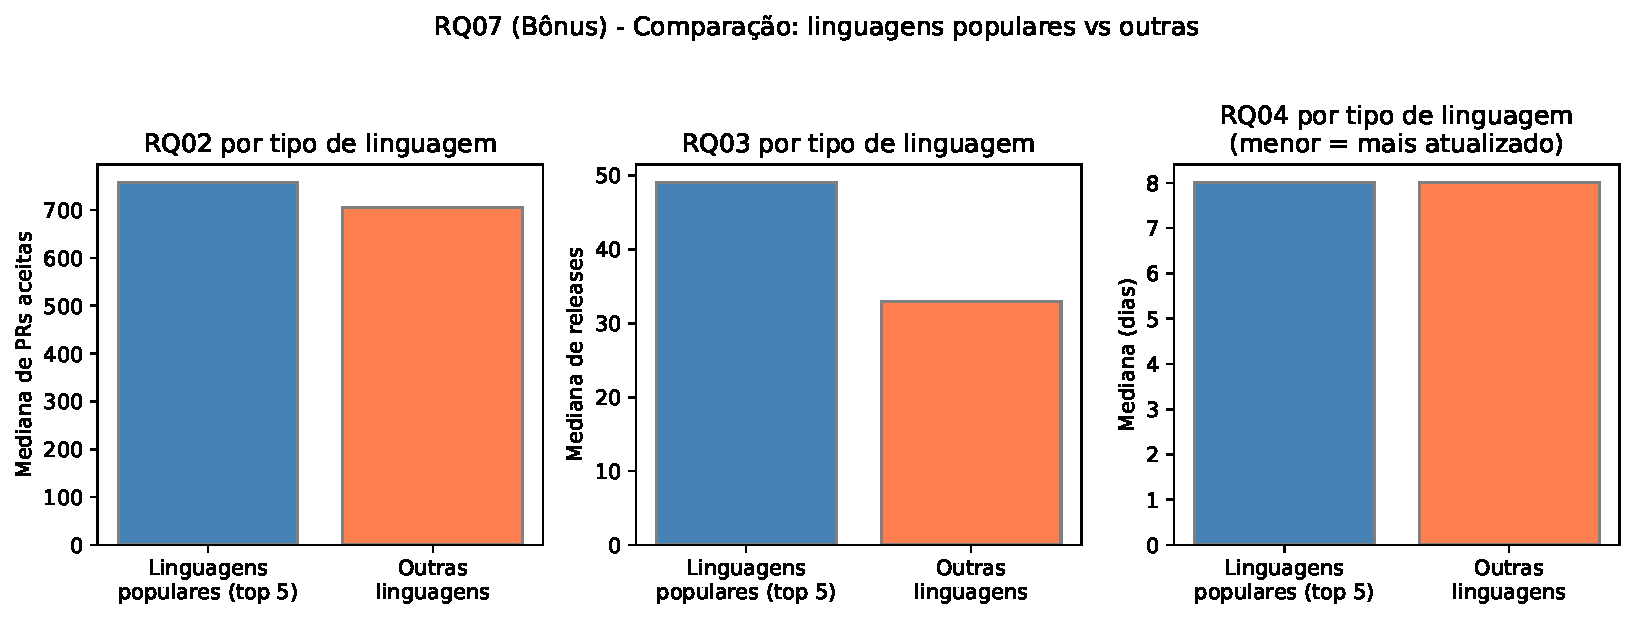
\includegraphics[width=\textwidth]{figuras/rq07_populares_vs_outras.pdf}
    \caption{RQ07 (Bônus): comparação das medianas entre repositórios em linguagens populares (top 5) e em outras linguagens. Menor mediana de ``dias desde atualização'' indica repositórios mais atualizados.}
    \label{fig:rq07-comparacao}
\end{figure}

\section{Discussão dos resultados}

\subsection*{Confronto das Questões-Pesquisa e Estatísticas}

Os dados revelaram que as expectativas iniciais foram em grande parte confirmadas, com nuances em algumas RQs.

\textbf{RQ 01 -- Sistemas populares são maduros/antigos?} A mediana de idade encontrada foi de \textbf{8,42 anos}. A hipótese foi \textbf{confirmada}: a maioria dos repositórios no top 1.000 é antiga o suficiente para ter acumulado comunidade e estrelas ao longo do tempo.

\textbf{RQ 02 -- Sistemas populares recebem muita contribuição externa?} A mediana de pull requests aceitas foi \textbf{736}. A hipótese foi \textbf{confirmada}: o volume de PRs aceitas é alto, indicando forte participação da comunidade.

\textbf{RQ 03 -- Sistemas populares lançam releases com frequência?} A mediana de releases foi \textbf{40}. A hipótese foi \textbf{parcialmente confirmada}: há uma base sólida de releases, embora a distribuição seja assimétrica (muitos repos com poucas ou zero releases formais, e outros com dezenas/centenas), o que puxa a mediana para um valor moderado.

\textbf{RQ 04 -- Sistemas populares são atualizados com frequência?} A mediana de dias desde a última atualização foi \textbf{8 dias}. A hipótese foi \textbf{confirmada}: repositórios populares tendem a ser atualizados com frequência (ordem de poucos dias).

\textbf{RQ 05 -- Sistemas populares são escritos nas linguagens mais populares?} A contagem por categoria (Tabela~\ref{tab:linguagens}) mostrou domínio de Python (200), TypeScript (160), JavaScript (116), Go (76) e Rust (54), além de 95 repos ``Sem linguagem'' (listas, docs, etc.). A hipótese foi \textbf{confirmada}: as linguagens mais adotadas no mercado e em ecossistemas open-source predominam.

\textbf{RQ 06 -- Sistemas populares possuem um alto percentual de issues fechadas?} A mediana da razão de issues fechadas (considerando apenas repositórios com issues) foi \textbf{87,7\%}. A hipótese foi \textbf{confirmada}: a maior parte das issues está resolvida e fechada, refletindo manutenção ativa.

\subsection*{Insights, Comparações e Gráficos}

A análise das linguagens primárias (RQ05) mostrou um domínio significativo de ecossistemas como JavaScript, Python, TypeScript, Go e Rust. Ao cruzar essas linguagens populares com as métricas de contribuição na \textbf{RQ07} (Figura~\ref{fig:rq07-comparacao}), observou-se que o grupo ``linguagens populares'' (top 5: Python, TypeScript, JavaScript, Sem linguagem, Go) apresenta mediana de PRs aceitas ligeiramente maior (757 vs 705) e mediana de releases maior (49 vs 33) que o grupo ``outras linguagens''. A mediana de dias desde a última atualização foi igual (8 dias) nos dois grupos. Assim, a hipótese do bônus é \textbf{parcialmente corroborada}: sistemas em linguagens mais populares recebem um pouco mais de contribuição externa e lançam mais releases em mediana; em relação à frequência de atualização, não houve diferença entre os grupos na mediana.

\section{Conclusão}

\subsection*{Tomada de Decisão e Resultado Conclusivo}
A análise dos 1.000 repositórios mais populares do GitHub demonstra que o sucesso e o engajamento massivo estão atrelados a \textbf{maturação no tempo} (mediana de idade de 8,42 anos), \textbf{alta contribuição externa} (mediana de 736 PRs aceitas), \textbf{manutenção ativa} (mediana de 8 dias desde a última atualização e 87,7\% de issues fechadas) e \textbf{uso de linguagens predominantes} (Python, TypeScript, JavaScript, Go). As hipóteses propostas foram em grande parte confirmadas. O bônus (RQ07) indicou que repositórios em linguagens mais populares tendem a ter mediana maior de PRs e de releases, sem diferença na frequência de atualização.

\subsection*{Sugestões Futuras}
Para trabalhos futuros, sugere-se a investigação de métricas complementares, como a correlação entre o número de forks e o tamanho da equipe de core developers, a adoção de testes automatizados nesses repositórios, e a análise temporal (evolução das medianas ao longo dos anos).

\end{document}
